\subsection{Architectures and Training}
\label{sec:training}

\begin{figure}
    \vspace*{-\figskipabove px}
    \centering
    \hspace*{-4px}
    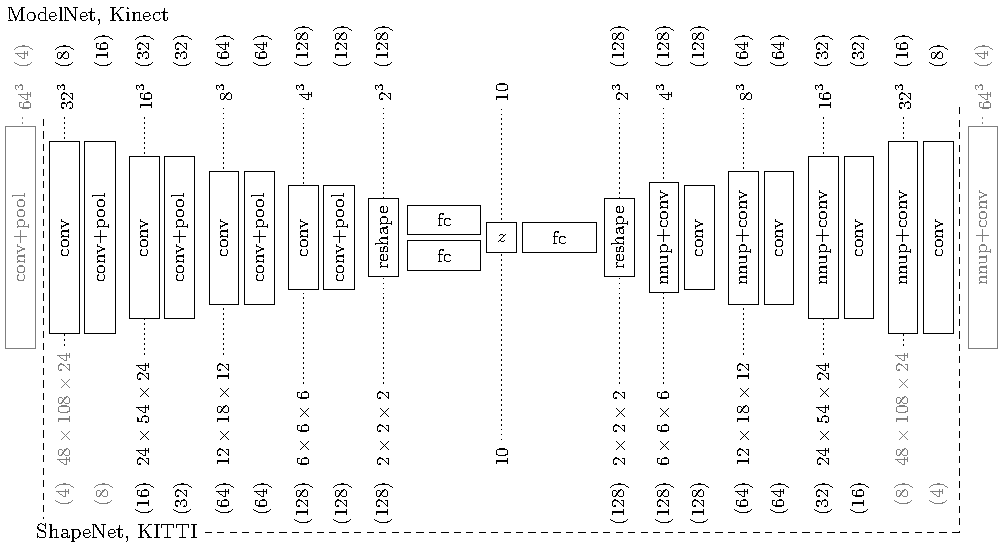
\includegraphics[width=1.025\linewidth]{fig_architectures}
    \vspace*{-12px}
    \caption{{\bf Network Architectures.} We use different resolutions for ShapeNet and KITTI as well as ModelNet and \Kinect (bottom and top, respectively). In both cases, architectures for higher resolutions employ one additional stage in the en- and decoder (in {\color{gray}gray}). Each convolutional layer is followed by $\text{ReLU}$ activations and batch normalization \citep{Ioffe2015ICML}; the window sizes for max pooling and nearest-neighbor upsampling can be derived from the context; the number of channels are given in parentheses.}
    \label{fig:architectures}
    \vspace*{-\figskipbelow px}
\end{figure}

As depicted in \figref{fig:architectures}, our network architectures are kept simple and shallow. Considering a resolution of $24 \ntimes 54 \ntimes 24$ voxels on ShapeNet and KITTI, the encoder comprises three stages, each consisting of two convolutional layers (followed by $\text{ReLU}$ activations and batch normalization \citep{Ioffe2015ICML}) and max pooling; the decoder mirrors the encoder, replacing max pooling by nearest neighbor upsampling. We consistently use $3^3$ convolutional kernels. We use a latent space of size $Q = 10$ and predict occupancy using Sigmoid activations.

We found that the shape representation has a significant impact on training. Specifically, learning both occupancy grids and SDFs works better compared to training on SDFs only. Additionally, following prior art in single image depth prediction \citep{Eigen2015ICCV,Eigen2014NIPS,Laina2016THREEDV}, we consider log-transformed, truncated SDFs (logTSDFs) for training: given a signed distance $y_i$, we compute $\text{sign}(y_i)\log(1 + \min(5, |y_i|))$ as the corresponding log-transformed, truncated signed distance. TSDFs are commonly used in the literature \citep{Newcombe2011ISMAR,Riegler2017THREEDV,Dai2017CVPRa,Engelmann2016GCPR,Curless1996SIGGRAPH} and the logarithmic transformation additionally increases the relative importance of values around the surfaces (\ie, around the zero crossing).

For training, we combine occupancy grids and logTSDFs in separate feature channels and randomly translate both by up to $3$ voxels per axis. Additionally, we use Bernoulli noise (probability $0.1$) and Gaussian noise (variance $0.05$). We use Adam \citep{Kingma2015ICLR}, a batch size of $16$ and the initialization scheme by \cite{Glorot2010AISTATS}. The shape prior is trained for $3000$ to $4000$ epochs with an initial learning rate of $10^{-4}$ which is decayed by $0.925$ every $215$ iterations until a minimum of $10^{-16}$ has been reached. In addition, weight decay ($10^{-4}$) is applied. For shape inference, training takes $30$ to $50$ epochs, and an initial learning rate of $10^{-4}$ is decayed by $0.9$ every $215$ iterations. For our learning-based baselines (see \secref{sec:baselines}) we require between $300$ and $400$ epochs using the same training procedure as for the shape prior. On the \Kinect dataset, where only $30$ training examples are available, we used $5000$ epochs. We use $\log \sigma^2 = -2$; weight the Kullback-Leibler divergence $\text{KL}$ (for \DVAE and (d)AML) with $\lambda =2, 2.5, 3$ with increasing resolution and use $\lambda = 1$ on KITTI. In addition, we reduce the weight in free space areas to one fourth on \noisy and KITTI to balance between occupied and free space. We implemented our networks in Torch \citep{Collobert2011NIPSWORK}.